\section{METODOLOGÍA SCRUM}

En el entorno empresarial actual, caracterizado por la volatilidad y la incertidumbre, la gestión de proyectos se ha convertido en un desafío crucial \autocite{sutherland2014scrum}. La metodología tradicional de cascada, con su enfoque lineal y rígido, a menudo resulta inadecuada para proyectos complejos y cambiantes. En este contexto, Scrum emerge como una alternativa ágil y flexible que permite a los equipos responder de manera efectiva a los cambios y entregar valor de forma incremental \autocite{schwaber2020guia}.

\subsection{DEFINICIÓN}

Scrum es un marco de trabajo ágil que proporciona una estructura para gestionar proyectos complejos \autocite{schwaber2020guia}. A diferencia de los enfoques tradicionales, Scrum se basa en ciclos iterativos e incrementales llamados Sprints, que permiten al equipo entregar resultados tangibles en períodos cortos de tiempo \autocite{rubin2012essential}. Scrum se enfoca en la colaboración, la adaptabilidad y la mejora continua, lo que lo convierte en una herramienta poderosa para abordar proyectos en entornos dinámicos \autocite{cohn2010suceeding}.

\subsection{ROLES}

Scrum define tres roles principales, cada uno con responsabilidades específicas \autocite{schwaber2020guia}:

\begin{itemize}
    \item \textbf{Product Owner:} Es el responsable de maximizar el valor del producto \autocite{cohn2010suceeding}. Sus responsabilidades incluyen:

    \begin{itemize}
        \item Definir y comunicar la visión del producto.
        \item Crear y mantener el Product Backlog, priorizando los elementos según el valor que aportan al negocio.
        \item Asegurar que el equipo de desarrollo comprenda los elementos del Product Backlog.
        \item Aceptar o rechazar el trabajo realizado al final de cada Sprint.
    \end{itemize}

    \item \textbf{Scrum Master:} Es el líder servidor del equipo Scrum y el responsable de garantizar que se siga el marco de trabajo de Scrum \autocite{rubin2012essential}. Sus responsabilidades incluyen:

    \begin{itemize}
        \item Facilitar los eventos de Scrum y ayudar al equipo a resolver problemas.
        \item Eliminar obstáculos que impidan el progreso del equipo.
        \item Proteger al equipo de interferencias externas.
        \item Promover la autogestión y la mejora continua del equipo.
    \end{itemize}

    \item \textbf{Equipo de Desarrollo:} Es un grupo autoorganizado y multifuncional responsable de entregar el producto \autocite{schwaber2020guia}. Sus responsabilidades incluyen:

    \begin{itemize}
        \item Planificar y estimar el trabajo a realizar en cada Sprint.
        \item Crear el incremento de producto "Hecho" al final de cada Sprint.
        \item Colaborar estrechamente para lograr el objetivo del Sprint.
        \item Asistir a los eventos de Scrum y participar activamente en ellos.
    \end{itemize}

    \item \textbf{Partes Interesadas (Stakeholders):} Son personas o grupos que tienen un interés en el resultado del proyecto \autocite{schwaber2020guia}. Pueden ser usuarios finales, clientes, patrocinadores, gerentes, etc. Es importante involucrar a las partes interesadas en el proceso de Scrum para garantizar que el producto satisfaga sus necesidades y expectativas.
\end{itemize}

\subsection{EVENTOS}

Scrum se estructura en torno a una serie de eventos que marcan el ritmo del proyecto \autocite{schwaber2020guia}:

\begin{itemize}
    \item \textbf{Sprint Planning:} El equipo planifica el trabajo a realizar durante el Sprint, seleccionando elementos del Product Backlog y definiendo un objetivo para el Sprint \autocite{rubin2012essential}.
    \item \textbf{Daily Scrum:} Reunión diaria de 15 minutos en la que el equipo sincroniza su trabajo y planifica el día \autocite{schwaber2020guia}.
    \item \textbf{Sprint Review:} El equipo presenta los resultados del Sprint a las partes interesadas y recibe retroalimentación \autocite{rubin2012essential}.
    \item \textbf{Sprint Retrospective:} El equipo reflexiona sobre el Sprint, identifica áreas de mejora y planifica cómo implementar cambios en el próximo Sprint \autocite{schwaber2020guia}.
\end{itemize}

\subsection{ARTEFACTOS}

Scrum utiliza tres artefactos principales para gestionar el trabajo y la información \autocite{schwaber2020guia}:

\begin{itemize}
    \item \textbf{Product Backlog:} Lista ordenada de todo lo que se necesita para mejorar el producto \autocite{cohn2010suceeding}. El Product Owner es responsable de su contenido y priorización.
    \item \textbf{Sprint Backlog:} Lista de elementos del Product Backlog seleccionados para el Sprint, junto con un plan para entregarlos \autocite{rubin2012essential}.
    \item \textbf{Incremento:} Resultado tangible del Sprint, que debe ser potencialmente entregable y cumplir con la Definición de Terminado del equipo \autocite{schwaber2020guia}.
\end{itemize}

\subsection{FLUJO DE TRABAJO}

El flujo de trabajo en Scrum se basa en ciclos iterativos llamados Sprints. Cada Sprint comienza con la planificación y termina con la revisión y la retrospectiva. Durante el Sprint, el equipo trabaja en los elementos del Sprint Backlog, realizando reuniones diarias para sincronizar su trabajo y adaptarse a los cambios. Al final del Sprint, el equipo entrega un Incremento del producto y reflexiona sobre cómo mejorar en el próximo Sprint.

\begin{figure}[H]
    \centering
    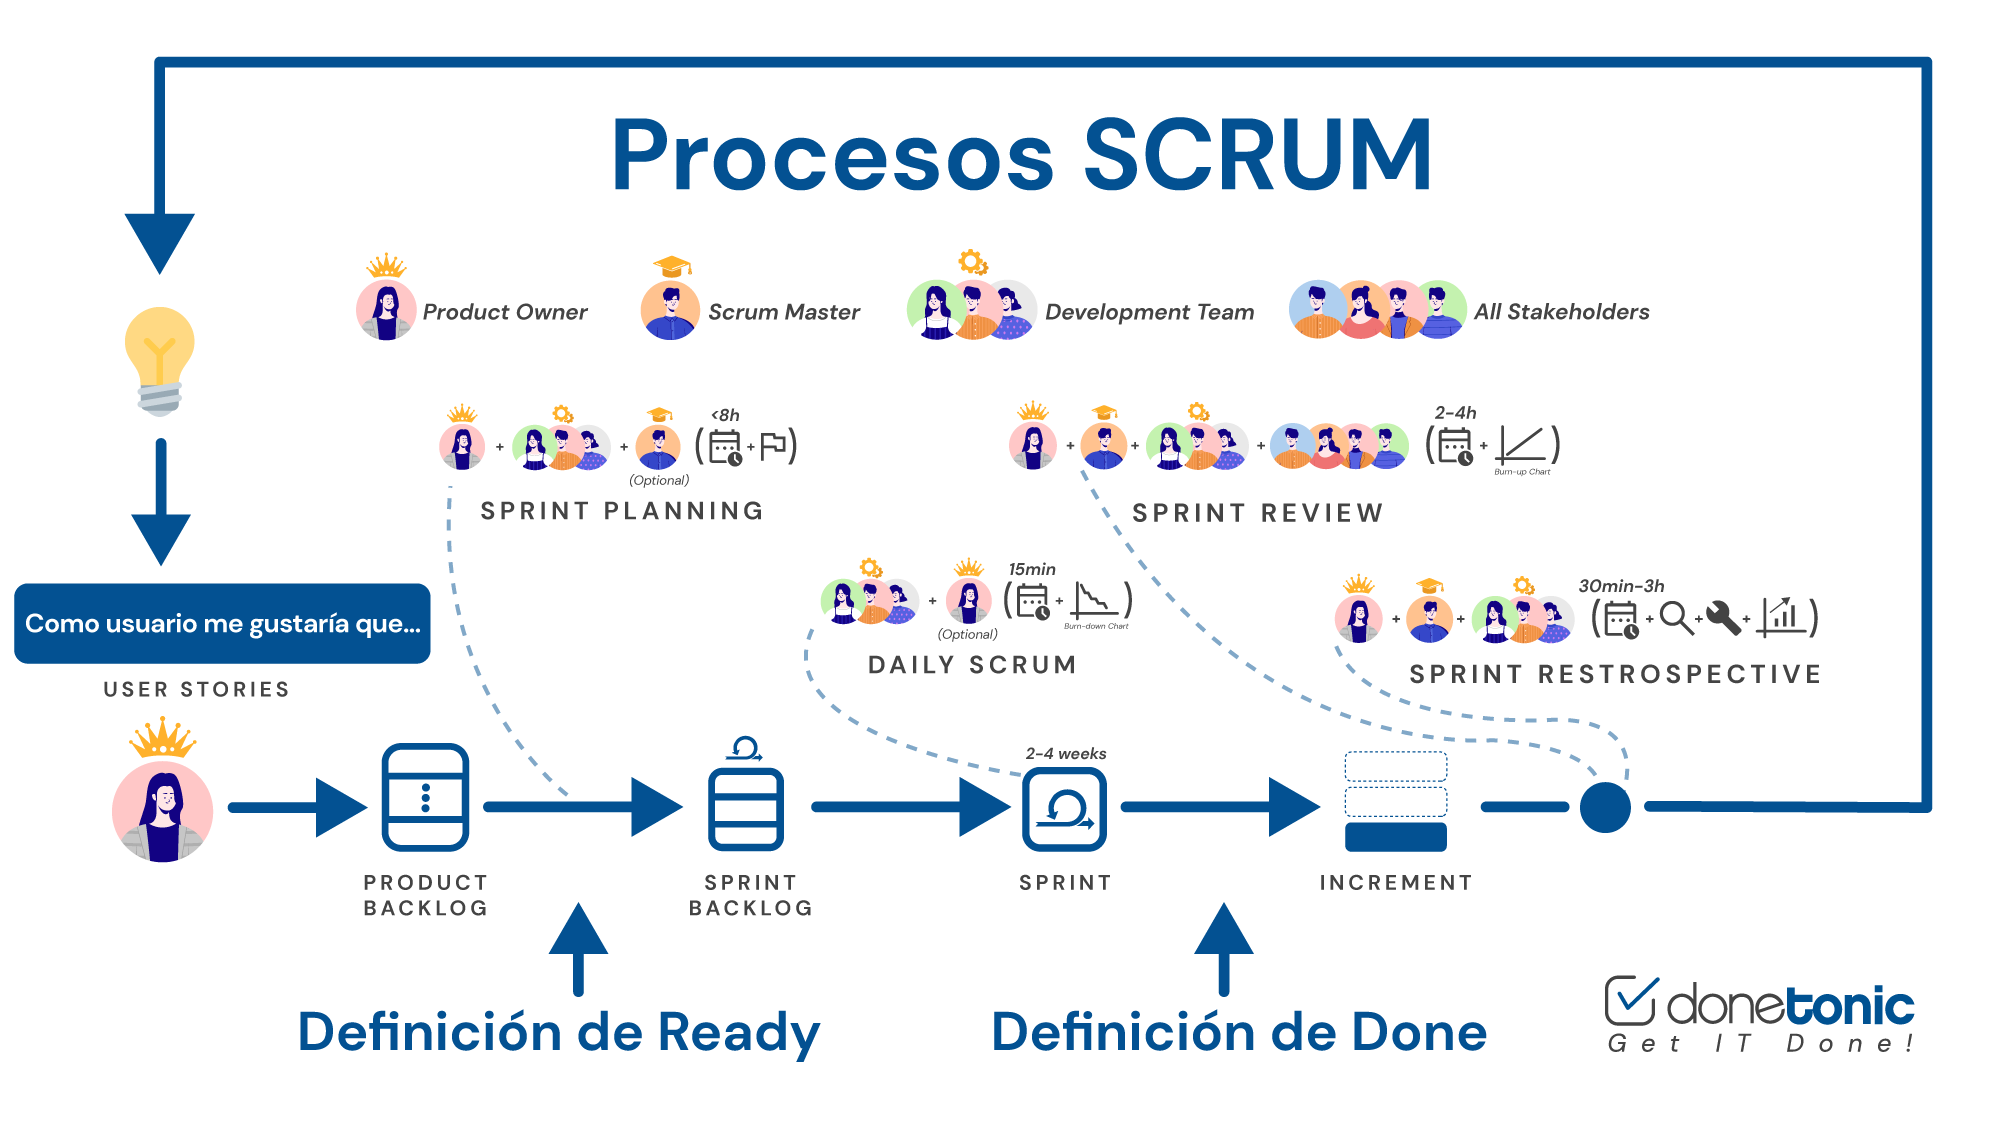
\includegraphics[scale=0.24]{imagenes/Procesos-SCRUM.png}
    \caption{Procesos SCRUM\\ Fuente: Elaboración propia}
\end{figure}

\subsection{CONCLUSIÓN}

Scrum ha demostrado ser una metodología eficaz para gestionar proyectos complejos en entornos cambiantes \autocite{sutherland2014scrum}. Su enfoque iterativo, colaborativo y centrado en el valor permite a los equipos entregar resultados de alta calidad de manera eficiente y adaptarse a los cambios del mercado. Al adoptar los roles, eventos y artefactos de Scrum, las organizaciones pueden mejorar su capacidad para gestionar proyectos y lograr sus objetivos de negocio \autocite{cohn2010suceeding}.
